\section{РАЗРАБОТАННОЕ РЕШЕНИЕ}

\subsection{Подход к решению задачи}

После консультации с врачом, работающим в отделении неотложной медицинской помощи, были выделены следующие критерии для эффективного решения задачи отображения страниц справочника:

\begin{itemize}
    \item интерфейс: основной принцип разработки интерфейса состоит в его интуитивной понятности, чтобы пользователи могли легко ориентироваться на страницах справочника. Все элементы управления должны быть расположены таким образом, чтобы их использование было интуитивно понятным и не требовало больших усилий;
    \item оптимизация информации: учитывая условия работы в отделении неотложной медицинской помощи, статьи справочника должны быть оптимизированы с точки зрения предоставления только самой важной и необходимой информации. Отсеивание избыточных данных и акцентирование внимания на ключевых сведениях позволит медицинскому персоналу быстро получать нужную информацию без необходимости тратить время на чтение больших объемов текста;
    \item группировка и функция поиска: для удобства навигации и быстрого доступа к нужным сведениям, статьи в справочнике должны быть сгруппированы по соответствующим категориям или темам. Также необходимо реализовать эффективную функцию поиска, которая позволит пользователям быстро находить нужные статьи. Поисковой механизм должен быть точным и эффективным, чтобы облегчить работу медицинского персонала в условиях неотложной помощи;
    \item функция добавления статей: для обеспечения актуальности и расширения информационной базы справочника, необходима возможность добавления новых статей. Эта функция должна предоставлять пользователю удобный интерфейс, где можно будет ввести заголовок, категорию, и внести основной текст статьи. Эта функция должна быть доступна только пользователям с соответствующими правами доступа;
    \item функция редактирования статей: для обновления информации в справочнике, пользователи с соответствующими правами доступа должны иметь возможность редактировать уже существующие статьи. Она позволит вносить изменения в текст статьи, обновлять связанные атрибуты (например, категорию или определение) и улучшать содержание для точности и актуальности данных. Интерфейс редактирования должен быть интуитивно понятным, позволяя пользователям легко найти и внести необходимые изменения в статьи;
    \item функция удаления статей: для поддержания надежности и актуальности информации в справочнике, необходимо предусмотреть функцию удаления статей, которая была бы доступна пользователям с соответствующими правами доступа. Также необходимо добавить подтверждение действия перед окончательным удалением статьи, чтобы пользователи могли избежать нежелательных ошибок;
    \item открытие страниц в новых вкладках: для обеспечения быстрого возврата к предыдущей открытой статье, страницы справочника должны открываться в новых вкладках браузера. Это позволит врачам легко переключаться между статьями, сохраняя контекст работы и экономя время на поиске и повторном открытии страниц.
\end{itemize}

Учитывая эти требования, при разработке интерфейса отображения страниц справочника необходимо обеспечить простоту использования, логичную структуру, адаптивность к различным устройствам и возможность интеграции с дополнительными функциональностями для облегчения работы пользователей и обеспечения удобства использования сервиса.

Алгоритм работы web-справочника включает следующие шаги:

\begin{itemize}
    \item осуществляется запрос на сервер, по которому происходит извлечение данных о заголовках и категориях статей из базы данных;
    \item по полученным данным все статьи группируются по категориям;   
    \item пользователь взаимодействует с интерфейсом web-справочника, вводя запросы в поисковую строку или выбирая категории и просматривая статьи из списка;
    \item введенные запросы и выбранные параметры передаются в соответствующие функции, которые обрабатывает запросы и выполняет соответствующие действия;
    \item программа осуществляет поиск данных, используя предопределенные алгоритмы поиска и фильтрации;
    \item при клике на заголовок статьи осуществляется запрос на сервер, по которому происходит извлечение данных о выбранной статье;
    \item полученные данные отображаются пользователю в удобном и понятном виде.
\end{itemize}

\subsection{Обоснование стека используемых технологий}

JavaScript является одним из самых популярных языков программирования, используемых для разработки web-приложений. Он является клиентским языком программирования, выполняющимся в браузере пользователя и позволяющим добавлять динамическое поведение к web-страницам. JavaScript обеспечивает множество возможностей для создания интерактивных и отзывчивых пользовательских интерфейсов \cite{JavaScript}.

JavaScript также обладает множеством других возможностей, которые делают его привлекательным для разработки web-приложений. Он поддерживает асинхронное программирование, что позволяет выполнять задачи без блокирования основного потока выполнения. JavaScript имеет множество встроенных функций и методов, которые упрощают манипуляцию с DOM (Document Object Model), обработку событий, отправку HTTP-запросов и многое другое.

В целом, JavaScript является мощным инструментом для разработки веб-приложений. С его помощью разработчики могут создавать интерактивные пользовательские интерфейсы, обрабатывать данные, взаимодействовать с сервером и использовать различные фреймворки и библиотеки, такие как React и Angular, для создания масштабируемых и производительных приложений.

При разработке клиентской части web-приложения выбор стоял между двумя фреймворками — React и Angular. Рассмотрим их подробнее:

React — это библиотека для разработки пользовательских интерфейсов, фокусирующаяся на создании компонентов. Он предоставляет мощные инструменты для управления состоянием и эффективного рендеринга обновлений. React использует JSX для объединения JavaScript и HTML-подобного синтаксиса \cite{React}.

Angular — это полноценный фреймворк для разработки web-приложений. Он предоставляет инструменты для создания компонентов, управления состоянием, маршрутизации, обработки событий и многое другое. Angular использует TypeScript и шаблоны HTML для создания приложений \cite{Angular}.

Сравним их:

\begin{itemize}
    \item размер и сложность: React является более легковесным и простым в освоении по сравнению с Angular. Angular имеет больший размер и более сложную структуру, что может потребовать больше времени для изучения и освоения;
    \item гибкость и расширяемость: React предоставляет большую гибкость и свободу в выборе других инструментов и библиотек, таких как маршрутизация или управление состоянием (Redux, MobX и другие). Angular предлагает широкий набор инструментов встроенно, что упрощает разработку приложений, но может быть менее гибким при необходимости использования сторонних решений;
    \item производительность: оба фреймворка обеспечивают хорошую производительность, но React, благодаря своему виртуальному DOM и механизму сравнения изменений, может быть более эффективным в обновлении компонентов.
\end{itemize}

Проанализировав преимущества и недостатки каждого фреймворка, выбор пал на React. В обоснование этого выбора следует отметить несколько причин:

\begin{itemize}
    \item легкость освоения и использования: React предоставляет простой и интуитивно понятный подход к разработке пользовательских интерфейсов. Его основной концепцией является создание компонентов, что позволяет разбить интерфейс на небольшие независимые блоки. Это упрощает понимание и модификацию кода, а также облегчает внедрение новых разработчиков в проект;
    \item эффективный рендеринг обновлений: React использует виртуальный DOM и механизм сравнения изменений, что позволяет эффективно обновлять только необходимые части интерфейса при изменении состояния. Это особенно полезно в условиях работы веб-справочника, где быстрое обновление данных и реакция на взаимодействие пользователя являются важными требованиями;
    \item обширная экосистема и сообщество: React имеет огромную экосистему, включающую библиотеки и инструменты для различных задач разработки, такие как маршрутизация, управление состоянием и тестирование. Это позволяет выбирать наиболее подходящие инструменты и расширения для вашего проекта. Кроме того, React обладает активным и развитым сообществом разработчиков, где можно получить поддержку, решить проблемы и узнать о лучших практиках;
    \item популярность и поддержка: React является одним из самых популярных инструментов для разработки пользовательских интерфейсов. Благодаря своей популярности, React имеет широкую поддержку и активное развитие. Это обеспечивает стабильность, надежность и постоянное обновление библиотеки.
\end{itemize}

Для взаимодействия приложения с сервером был выбран REST API (Representational State Transfer Application Programming Interface) — это архитектурный стиль для разработки web-сервисов. REST API предоставляет набор принципов, которые определяют, как взаимодействовать с web-сервисом. Он использует стандартные HTTP-методы, включая GET, POST и DELETE, для выполнения операций над ресурсами. REST API обеспечивает гибкость и масштабируемость взаимодействия между клиентом и сервером, позволяя выполнять различные операции, такие как создание, чтение, обновление и удаление данных \cite{API}.

При проектировании и разработке web-приложений, использование API-запросов, таких как GET- и POST-запросы, имеет несколько преимуществ:
\begin{itemize}
    \item получение данных с сервера: использование GET-запросов позволяет получать данные с сервера, необходимые для работы и отображения в приложении. Это может быть информация о пользователях, продуктах, новостях или любых других данных, которые приложение должно получать извне. POST-запросы, в свою очередь, используются для отправки данных на сервер, например, при создании новых записей или отправке форм;
    \item асинхронность и отзывчивость: и GET-запросы, и POST-запросы выполняются асинхронно, что позволяет приложению продолжать работу, пока данные отправляются или обрабатываются на сервере. Это поддерживает отзывчивый пользовательский интерфейс и позволяет пользователям взаимодействовать с приложением без задержек;
    \item обновление данных: POST-запросы часто используются для обновления данных на сервере. Например, при редактировании информации о пользователе или изменении статуса заказа. Отправка POST-запроса с обновленными данными позволяет приложению синхронизироваться с сервером и обновить информацию;
    \item удобство и простота использования: GET- и POST-запросы являются одними из наиболее распространенных типов запросов и относительно легко реализуются в коде приложения. Для выполнения запросов на сервер существуют различные библиотеки и инструменты, такие как Fetch API или axios, которые упрощают отправку запросов и обработку полученных данных;
    \item кэширование: и GET-запросы, и POST-запросы могут использовать кэширование для оптимизации производительности. Однако обычно POST-запросы не кэшируются, поскольку они могут иметь побочные эффекты на сервере, такие как изменение данных.
\end{itemize}

Также была выбрана библиотека компонентов для React — MUI \cite{MUI}. Она предоставляет готовые стилизованные компоненты, которые соответствуют принципам Material Design. Использование MUI упростит разработку, добавление стилей и создание современного и эстетически привлекательного интерфейса.  Библиотека MUI предлагает широкий набор компонентов, таких как кнопки, формы, таблицы, диалоги, навигационные панели и многое другое. Каждый компонент разработан с учетом принципов Material Design, что обеспечивает современный и согласованный внешний вид пользовательского интерфейса.

Одной из ключевых особенностей MUI является ее гибкость и настраиваемость. Компоненты MUI могут быть легко настроены и адаптированы под конкретные требования проекта. Они также поддерживают темизацию, что позволяет изменять внешний вид компонентов, чтобы они соответствовали дизайну проекта.

MUI обладает активным сообществом разработчиков и постоянно обновляется, предоставляя новые компоненты и функциональность. Она также интегрируется с другими популярными инструментами и библиотеками, такими как React Router и Redux, что делает ее идеальным выбором для разработки современных web-приложений на базе React.

Для создания макета было выбрано web-приложение Figma \cite{Figma}. Figma - это web-приложение для дизайна интерфейсов, которое позволяет дизайнерам и командам работать над созданием и прототипированием пользовательских интерфейсов. Figma предоставляет инструменты для создания макетов, иллюстраций, прототипов и совместной работы над проектами в режиме реального времени.

Основная особенность Figma заключается в его возможности работать на разных платформах и быть доступным через web-браузер без необходимости установки дополнительного программного обеспечения. Это позволяет дизайнерам и командам с легкостью сотрудничать над проектами, делиться макетами и получать обратную связь в режиме реального времени.

Также Figma обладает широким набором инструментов для создания и редактирования дизайна, включая возможность работы с векторной графикой, добавления интерактивных элементов и создания анимаций. Он также предлагает функции комментирования и обсуждения, что упрощает процесс сотрудничества и согласования изменений в проекте.

Все это позволяет создать современный и интуитивно понятный интерфейс, что особенно важно для удобства использования web-справочника.

\subsection{Описание программной разработки}

В рамках программной разработки функционального web-справочника в приложении электронного заполнения медицинских карт было выполнено несколько шагов.

Сначала был разработан макет. С помощью инструмента Figma был создан макет будущей страницы справочника, представленный на рисунке~\ref{fig:page-model}, на котором расположены все необходимые элементы, такие как статьи, разделенные по категориям, и поисковая строка.

\begin{figure}
  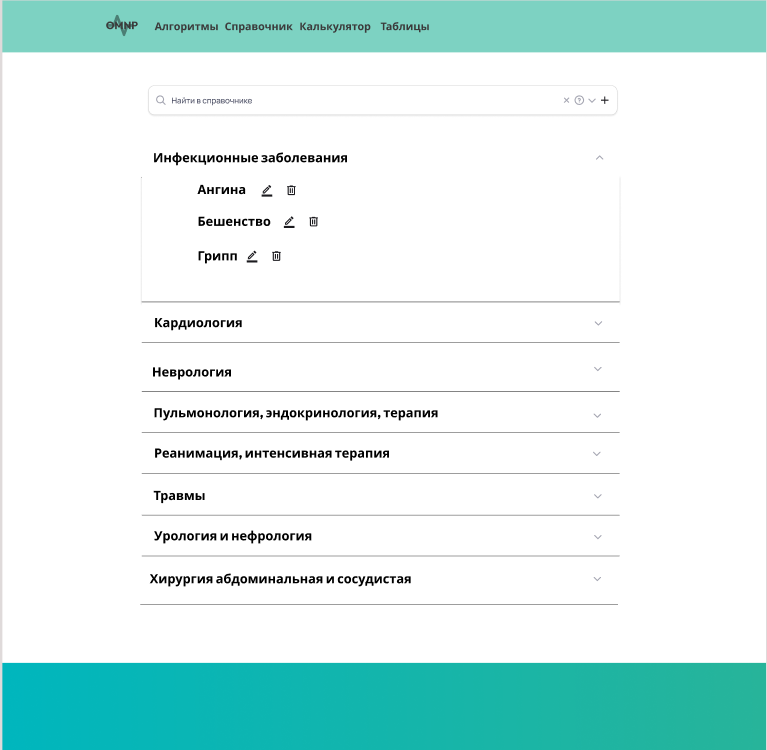
\includegraphics[scale=0.5]{styles/diploma/inc/Макет.png}
  \caption{Макет страницы справочника}
  \label{fig:page-model}
\end{figure}

Затем была проведена подготовка справочных данных. Консультирующий врач предоставил распечатанные примеры справочных материалов, представленные на рисунке~\ref{fig:ex-ref}, которые были использованы для составления информации о болезнях в формате определения, инкубационного периода (если есть), симптомов, форм заболевания (если есть). Дополнительно, информация была взята с сайтов <<Медицинская энциклопедия>>\cite{Encyclopedia}, <<Справочник MSD>>\cite{MSD} и телеграм-бота <<PARAMEDIC (шпаргалки)>>\cite{Paramedic}. Все справочные данные проверены и подтверждены консультирующим врачом.

\begin{figure}
  
\includegraphics[scale=0.5]{styles/diploma/inc/ex-ref.png}
  \caption{Пример распечатанного справочного материала}
  \label{fig:ex-ref}
\end{figure}

Для полной реализации проекта и разработки функционала, был создан проект на платформе GitLab, включающий все необходимые компоненты для электронного заполнения медицинских карт. Основная разработка функционала справочника происходила в папке <<src/pages/feature-pages/dictionary>>.

В рамках разработки был создан компонент ArticleModel.jsx, который содержит функцию createArticleData. Эта функция принимает заголовок статьи и данные из API-ответа и возвращает структурированные данные о статье, которые затем используются для ее отображения на странице.

На следующем рисунке~\ref{src:src2} показан листинг, который содержит функцию createArticleData:

 \begin{figure}
 \begin{lstlisting}[language=Python]
export const createArticleData = (title, data) => {
    const { tag, description, symptomps, period, forms } = data[title];
    const formDescriptions = data[title]['form descriptions'];
    const formSymptoms = data[title]['form symptomps'];
  
    return {
      tag,
      title,
      description,
      symptomps,
      period,
      forms,
      formDescriptions,
      formSymptoms,
    };
  };
\end{lstlisting}
\caption{Функция createArticleData}
\label{src:src2}
\end{figure}

Затем был создан компонент ArticlePage.jsx, который отображает текст статьи. При загрузке страницы, с помощью хука useEffect, происходит получение данных статьи из sessionStorage. Если данные уже были сохранены, то они отображаются на странице. В противном случае выводится сообщение о том, что статья не найдена.

На главной странице справочника присутствует поиск по названию статьи, кнопка добавления новой статьи и аккордеон, заголовками которого выступают категории, а содержимым являются статьи, соответствующие этим категориям. У каждой статьи находятся кнопки редактирования и удаления. Эти функции были реализованы с использованием компонентов MUI (Material-UI). При изменении значения поиска происходит фильтрация статей и категорий. Также присутствует возможность сворачивания/разворачивания всех категорий с помощью кнопки. При клике на статью происходит открытие новой вкладки с полной статьей или перенаправление на страницу <<Статья не найдена>>, если статья отсутствует.

Для обеспечения адресации страниц справочника использовался React Router: была реализована маршрутизация и подключены компоненты для каждой страницы, включая страницу справочника.

После завершения разработки интерфейса в соответствии с макетом, был добавлен файл mockData.json, содержащий пример данных, которые будут передаваться с сервера. После тестирования приложения с этими данными, была настроена связь web-приложения с удаленным сервером с использованием REST API. В моем проекте для получения медицинских данных с сервера необходимо использовать GET-запрос. При загрузке приложения, с помощью функции useEffect, происходит отправка асинхронного запроса POST на адрес <<http://188.225.78.148/api/v1/>>. В заголовке запроса также передается токен CSRF для авторизации. Полученные данные в формате JSON обрабатываются и структурируются с использованием функции createArticleData. Эта функция принимает заголовок статьи и данные из API-ответа, а затем извлекает необходимую информацию, такую как категория, описание, симптомы, период, формы и т.д. Сначала мы используем GET-запрос для получения информации обо всех парах "заголовок статьи":"категория", которые есть на сервере. С помощью этих данных мы формируем аккордеоны. Когда пользователь нажимает на заголовок статьи, эта статья открывается в новой вкладке. Затем используется второй GET-запрос, в который передается заголовок статьи. На выходе мы получаем объект articleData, который содержит структурированную информацию о выбранной статье. Затем мы выводим эту информацию на странице.

Для добавления новой статьи используется POST-запрос, в который передаются параметры <<name>> (название заболевания), <<tag>> (категория заболевания), <<description>> (описание заболевания), <<period>> (продолжительность болезни или ее инкубационный период), <<symptoms>> (симптомы заболевания), <<forms>> (формы заболевания), <<forms descriptions>> (описания форм заболевания), <<forms symptomps>> (симптомы форм заболевания). Параметры <<name>> и <<tag>> не могут быть пустыми. Для удаления статьи используется метод DELETE, в который передается название статьи. Для редактирования статьи, используется форма, содержащая такие же параметры, как при добавлении новой статьи. При нажатии на кнопку <<Сохранить>>, если поля <<name>> и <<tag>> не пустые, происходит запрос DELETE, в который передается название статьи, которую редактировали, а затем происходит POST-запрос, в который передаются параметры, переданные в форме редактирования статьи. Если хотя бы одно из полей <<tag>> или <<name>> пустое, то форма запретит сохранение такой статьи.

Такая интеграция с удаленным сервером через REST API позволяет приложению получать актуальные медицинские данные и обновлять базу данных в соответствии с внесенными изменениями. Это обеспечивает актуальность и достоверность информации в web-справочнике, а также позволяет медицинским работникам скорой помощи оперативно получать необходимую информацию для принятия решений.

В результате программной разработки был создан функциональный web-справочник в приложении для электронного заполнения медицинских карт. Этот справочник предоставляет возможность пользователям осуществлять поиск и отображение медицинской информации, а также функции по добавлению, редактированию и удалению статей, значительно упрощая процесс заполнения медицинских карт и обеспечивая доступ к необходимым справочным материалам.
